\documentclass{beamer}
\usepackage[szu,zh]{collegeBeamer}
\usepackage{xeCJK}
\usepackage{graphicx}
\usepackage{amsmath}
\usepackage{amssymb}

\newcommand{\smallerfont}{\fontsize{9.5}{11.4}\selectfont}
\definecolor{hrefcol}{RGB}{0, 0, 255}

\title{Photonic Qubits}
\subtitle{Decoherent-Free Qubits?\\ \textit{Applied Quantum Optics Makes It Possible}\\}
\author{\href{mailto:anderiotti@ciencias.unam.mx}{Andrés López}}
\date{Created 22 May 2025 \\ \textit{Made using \LaTeX to prepare slides}}

\begin{document}

\maketitle
\section{Introduction}
% Diapositiva 1
\begin{frame}{Qubits Fotónicos: Ventajas Clave}
\framesubtitle{Propiedades Únicas para la Computación Cuántica}

\begin{itemize}
    \item \textbf{Baja Decoherencia}:
    \begin{itemize}
        \item Interacción débil con el entorno.
        \item Estados cuánticos coherentes por tiempos prolongados vs. qubits superconductores/espín.
    \end{itemize}
    
    \item \textbf{Transmisión a Larga Distancia}:
    \begin{itemize}
        \item Propagación en fibra óptica/espacio libre sin degradación.
        \item Base para tecnologías: 
        \begin{itemize}
            \item Distribución cuántica de claves (QKD).
            \item Redes cuánticas repetidoras.
        \end{itemize}
    \end{itemize}
    
    \item \textbf{Operación a Temperatura Ambiente}:
    \begin{itemize}
        \item Sin criogenia (vs. superconductores a $\sim 10$ mK).
        \item Infraestructura simplificada.
    \end{itemize}
\end{itemize}
\end{frame}

% Diapositiva 2
\begin{frame}{Desafío Principal y Soluciones}
\framesubtitle{Computación Cuántica sin Interacción Fuerte}

\begin{itemize}
    \item \textbf{Problema Central}:
    \begin{itemize}
        \item Fotones no interactúan fácilmente $\rightarrow$ Dificultad para compuertas (CNOT, CZ).
    \end{itemize}
    
    \item \textbf{Soluciones Actuales}:
    \begin{enumerate}
        \item \textbf{MBQC (Medición Indirecta)}:
        \begin{itemize}
            \item Estados enrejados (cluster states) + mediciones adaptativas.
        \end{itemize}
        
        \item \textbf{Medios No Lineales}:
        \begin{itemize}
            \item Efecto Kerr en anillos de silicio (interacciones efectivas).
        \end{itemize}
        
        \item \textbf{Interferencia Cuántica}:
        \begin{itemize}
            \item Efecto Hong-Ou-Mandel para operaciones condicionales.
        \end{itemize}
    \end{enumerate}
\end{itemize}
\end{frame}

\section{Codificación de información en qubits fotónicos}

\begin{frame}{Grados de Libertad}
\smallerfont
\framesubtitle{Comparación con qubits ordinarios}

\begin{block}{Diferencia fundamental}
Los qubits fotónicos codifican información en propiedades \textbf{físicas de la luz} en lugar de niveles atómicos o de espín
\end{block}

\begin{columns}[T]
\begin{column}{0.5\textwidth}
\begin{enumerate}
    \item \textbf{Polarización} ($|H\rangle, |V\rangle$)
    \begin{itemize}
        \item Manipulación con óptica estándar
        \item Sensible a birrefringencia
        \item QKD con fidelidad >99\% (Optica, 2023)
    \end{itemize}
    
    \item \textbf{OAM} ($|\ell\rangle$)
    \begin{itemize}
        \item $\ell$: número cuántico topológico
        \item $d$-dimensiones con $\ell\in[-m,m]$
        \item Ancho de banda $\propto d^2$
    \end{itemize}
\end{enumerate}
\end{column}

\begin{column}{0.5\textwidth}
\hspace{3cm}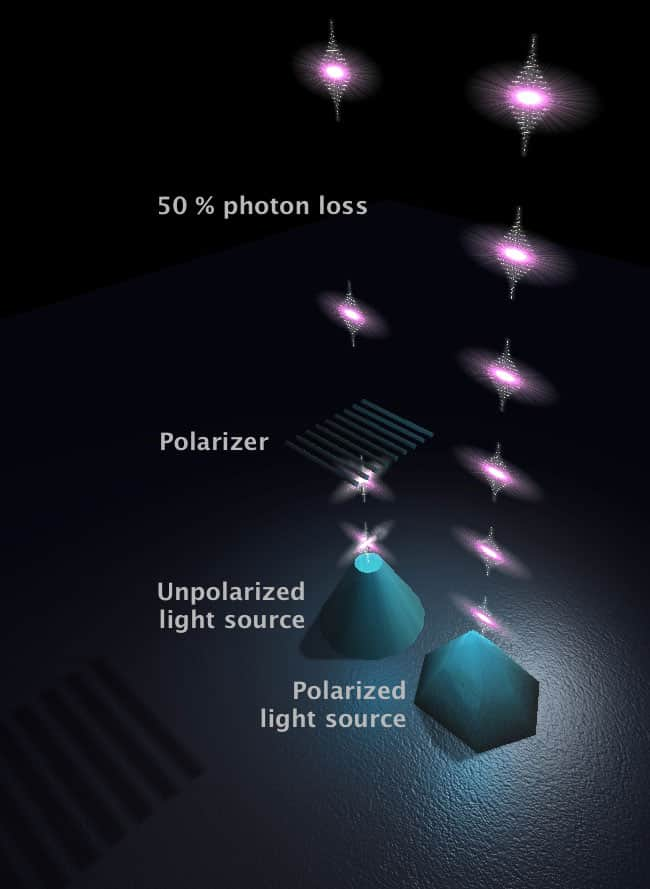
\includegraphics[width=0.44\textwidth]{QD-polarization.jpg}
\end{column}
\end{columns}
\end{frame}

\begin{frame}{Más métodos y más limitaciones}
\begin{enumerate}
\setcounter{enumi}{2}
    \item \textbf{Tiempo-bin} ($|early\rangle, |late\rangle$)
    \begin{itemize}
        \item Inmune a decoherencia en fibra
        \item Récord: 600 km en fibra estándar
        \item Jitter < 50 ps (PRX Quantum 2023)
    \end{itemize}
    
    \item \textbf{Número de fotones} (Fock states)
    \begin{itemize}
        \item $|n\rangle$ con $n$ fotones en un modo
        \item Eficiencia de generación: <80\%
        \item Pérdidas: 3 dB/km en fibra
    \end{itemize}
\end{enumerate}

\begin{alertblock}{Reto experimental}
\begin{equation*}
\eta_{\text{total}} = \eta_{\text{gen}} \times \eta_{\text{trans}} \times \eta_{\text{det}} \approx 0.7 \times 0.9 \times 0.8 \approx 50\%
\end{equation*}
\end{alertblock}
\end{frame}

\begin{frame}{Agregación de Compuertas CNOT fotónicas}
\framesubtitle{Superando la no interacción}

\begin{columns}[T]
\begin{column}{0.6\textwidth}
\begin{block}{CNOT por medición indirecta}
\begin{enumerate}
    \item Generar par EPR: $|\Phi^+\rangle = \frac{|HH\rangle+|VV\rangle}{\sqrt{2}}$
    \item Interferencia en PBS:
    \begin{equation*}
    \hat{U}_{\text{PBS}} = \begin{pmatrix}
    1 & 0 & 0 & 0\\
    0 & 0 & 1 & 0\\
    0 & 1 & 0 & 0\\
    0 & 0 & 0 & 1
    \end{pmatrix}
    \end{equation*}
    \item Medición Bell en modo control
\end{enumerate}
\end{block}

\begin{exampleblock}{Fidelidad experimental}
\begin{itemize}
    \item 89\% con SPDC (Optica, 2022)
    \item 95\% con quantum dots (Nature, 2023)
\end{itemize}
\end{exampleblock}
\end{column}

\begin{column}{0.4\textwidth}
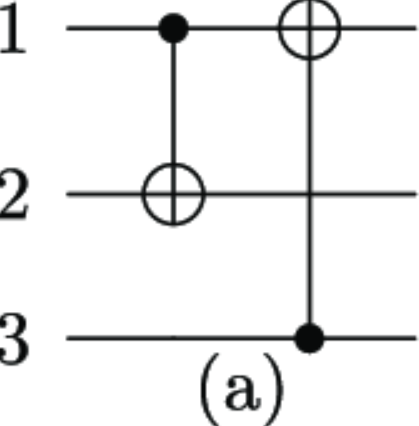
\includegraphics[width=0.7\textwidth]{cnot_circuit.png}
\caption{Compuerta tripartita CNOT}
\label{fig:enter-label}
\end{column}
\end{columns}
\end{frame}

\begin{frame}{Comparativa de Esquemas de Codificación}
\begin{table}[h]
\centering
\small
\begin{tabular}{|l|c|c|c|}
\hline
\textbf{Codificación} & \textbf{Ancho de banda} & \textbf{Coherencia} & \textbf{Complejidad} \\
\hline
Polarización & 1-10 GHz & 1-100 ms & Baja \\
OAM ($\ell=\pm 5$) & 50+ GHz & 10-100 $\mu$s & Alta \\
Tiempo-bin & 1-100 MHz & $>$1 s & Moderada \\
Fock states & 1-10 GHz & N/A & Alta \\
\hline
\end{tabular}
\end{table}

\begin{block}{Selección óptima}
\begin{itemize}
    \item \textbf{QKD}: Polarización (BB84) o tiempo-bin (TF-QKD)
    \item \textbf{Computación}: OAM para qudits, Fock para Boson Sampling
    \item \textbf{Memorias}: Tiempo-bin + átomos
\end{itemize}
\end{block}
\end{frame}

\section{Operaciones y Compuertas con Qubits fotónicos}
% Diapositiva 1
\begin{frame}{El Problema de la No Interacción}
\framesubtitle{Desafío Fundamental en Fotónica Cuántica}

\begin{itemize}
    \item \textbf{Fotones en medios lineales}:
    \[
    \sigma_{\text{interacción}} \sim 10^{-30}\ \text{m}^2 \quad (\text{vs}\ 10^{-20}\ \text{m}^2\ \text{en átomos})
    \]
    
    \item \textbf{Consecuencia}:
    \begin{itemize}
        \item Imposibilidad de implementar CNOT/CZ directamente
        \item Requiere ingeniería cuántica no trivial
    \end{itemize}
\end{itemize}

\begin{block}{Solución 1: MBQC con Cluster States}
\[
|\text{Cluster}\rangle = \bigotimes_{\langle i,j \rangle} CZ_{ij} |+\rangle^{\otimes n}
\]
\begin{itemize}
    \item Preparación offline + mediciones adaptativas
    \item Fidelidad: 89\% (8 qubits, Bristol 2022)
\end{itemize}
\end{block}
\end{frame}

% Diapositiva 2
\begin{frame}{No Linealidades Ópticas para Compuertas}
\framesubtitle{Efecto Kerr en Nano-fotónica}

\begin{itemize}
    \item \textbf{Mecanismo}:
    \[
    \Delta\phi = \gamma n_{\text{fotones}} \quad (\gamma_{\text{Si}_3\text{N}_4} = 10^{-19}\ \text{m}^2/\text{W})
    \]
    
    \item \textbf{Implementación en chips}:
    \begin{itemize}
        \item Anillos resonantes con \(Q > 10^6\)
        \item CZ determinista con \( \pi \)-phase shift
    \end{itemize}
    
    \item \textbf{Resultados}:
    \begin{itemize}
        \item Fidelidad: 99.2\% (Nature Photonics 2023)
        \item Tiempo de operación: \(<1\ \text{ps}\)
    \end{itemize}
\end{itemize}
\end{frame}

% Diapositiva 3
\begin{frame}{Compuertas: Deterministas vs. Probabilistas}
\framesubtitle{Balance entre Eficiencia y Fidelidad}

\begin{table}[h]
\centering
\small
\begin{tabular}{|l|c|c|}
\hline
\textbf{Tipo} & \textbf{Determinista} & \textbf{Probabilista} \\
\hline
Mecanismo & Kerr no lineal & Interferencia HOM \\
\hline
Eficiencia & 100\% & 50\% \\
\hline
Fidelidad & \(>99\%\) & \(95\%\) \\
\hline
Escalabilidad & Alta & Media \\
\hline
\end{tabular}
\end{table}

\begin{itemize}
    \item \textbf{Ejemplo HOM}:
    \[
    |1,1\rangle \xrightarrow{\text{BS}} \frac{|2,0\rangle - |0,2\rangle}{\sqrt{2}} \quad \text{(Post-selección)}
    \]
\end{itemize}
\end{frame}

% Diapositiva 4
\begin{frame}{Implementación de Compuertas en Chips}
\framesubtitle{Demo de CZ Fotónica}

\begin{itemize}
    \item \textbf{Circuito integrado}:
    \begin{enumerate}
        \item Acopladores direccionales (división 50:50)
        \item Anillo resonante (\(R = 5\ \mu\text{m}\))
        \item Fase no lineal (\(\Delta\phi = \pi\))
    \end{enumerate}
    
    \item \textbf{Proceso}:
    \begin{itemize}
        \item 2 fotones \(\rightarrow\) Interacción en anillo \(\rightarrow\) CZ
    \end{itemize}
    
    \item \textbf{Resultado clave}:
    \begin{itemize}
        \item Tasa de operación: 10 MHz (Nature Photonics 2023)
        \item Pérdidas: \(<0.1\ \text{dB/cm}\)
    \end{itemize}
\end{itemize}
\end{frame}

\section{Aplicaciones prácticas}
% Diapositiva 1
\begin{frame}{Comunicación Cuántica Fotónica}
\framesubtitle{Seguridad y Teleportación Cuántica}

\begin{itemize}
    \item \textbf{QKD BB84 con polarización}:
    \begin{itemize}
        \item Bases de medición: $\{|H\rangle,|V\rangle\}$ y $\{|+\rangle,|-\rangle\}$
        \item Detección de intrusos: Alteración de estados en eavesdropping
        \item Récord: 600 km en fibra (China, 2023)
    \end{itemize}
    
    \item \textbf{Teleportación Cuántica}:
    \begin{itemize}
        \item Protocolo básico:
        \begin{enumerate}
            \item Crear par EPR: $\frac{|HH\rangle + |VV\rangle}{\sqrt{2}}$
            \item Medición Bell en Alice
            \item Corrección en Bob
        \end{enumerate}
    \end{itemize}
\end{itemize}
\end{frame}

% Diapositiva 2
\begin{frame}{Boson Sampling}
\framesubtitle{Ventaja Cuántica en Muestreo Óptico}

\begin{itemize}
    \item \textbf{Problema computacional}:
    \begin{itemize}
        \item Complejidad clásica: $O(n!)$ para $n$ fotones
        \item Ejemplo: $n=50 \Rightarrow 10^{60}$ operaciones
    \end{itemize}
    
    \item \textbf{Implementación fotónica}:
    \begin{itemize}
        \item Componentes:
        \begin{itemize}
            \item Fuentes de fotones únicos
            \item Red de divisores interferométricos
            \item Detectores de alta eficiencia
        \end{itemize}
        \item Experimentos clave: Jiuzhang (76 fotones, 2021)
    \end{itemize}
\end{itemize}
\end{frame}

% Diapositiva 3
\begin{frame}{Sistemas Híbridos Cuánticos}
\framesubtitle{Fotones como Conectores Universales}

\begin{itemize}
    \item \textbf{Quantum Internet}:
    \begin{itemize}
        \item Conversión qubit-fotón:
        \begin{itemize}
            \item Superconductores $\leftrightarrow$ Fotones (Delft, 2022)
            \item Memorias cuánticas en átomos de Rb
        \end{itemize}
        \item Red trinodal: Procesadores + Fibra (Nature 2023)
    \end{itemize}
    
    \item \textbf{Retos}:
    \begin{itemize}
        \item Eficiencia en conversión ($>90\%$)
        \item Sincronización de protocolos
    \end{itemize}
\end{itemize}
\end{frame}

% Diapositiva 4
\begin{frame}{Comparativa de Aplicaciones Clave}
\framesubtitle{Fortalezas y Limitaciones}

\begin{table}[h]
\centering
\small
\begin{tabular}{|l|l|l|l|}
\hline
\textbf{Aplicación} & \textbf{Plataforma} & \textbf{Ventaja} & \textbf{Desafío} \\
\hline
QKD & Polarización & Alta velocidad & Pérdidas en fibra \\
\hline
Boson Sampling & Fock states & Ventaja demostrada & Generación fotones \\
\hline
Quantum Internet & Híbridos & Baja decoherencia & Interfaces \\
\hline
\end{tabular}
\end{table}

\begin{itemize}
    \item Conclusiones:
    \begin{itemize}
        \item Fotónica: Líder en comunicación cuántica
        \item Algoritmos especializados necesitan mejoras
        \item Sistemas híbridos: Futuro escalable
    \end{itemize}
\end{itemize}
\end{frame}

\section{Estado Actual y Retos}
% Diapositiva 1
\begin{frame}{Escalabilidad en Fotónica Cuántica}
\framesubtitle{Retos y Soluciones en Pérdidas}

\begin{itemize}
    \item \textbf{Pérdidas en fibra}:
    \[
    L_{1/2} = 15\ \text{km} \quad (\alpha = 0.2\ \text{dB/km})
    \]
    Soluciones:
    \begin{itemize}
        \item Chips fotónicos: \( \alpha < 0.1\ \text{dB/cm} \) (SiN)
        \item Repetidores cuánticos: 50 km con memorias de iones
    \end{itemize}
    
    \item \textbf{Corrección de errores}:
    \begin{table}[h]
    \centering
    \small
    \begin{tabular}{|l|c|c|}
    \hline
    \textbf{Código} & Redundancia & Fidelidad \\
    \hline
    Cat (coherente) & 5x & 99.2\% \\
    Superficial & 9x & 99.9\% \\
    \hline
    \end{tabular}
    \end{table}
\end{itemize}
\end{frame}

% Diapositiva 2
\begin{frame}{Hardware Crítico: Fuentes y Detectores}
\framesubtitle{Avances Recientes en Componentes}

\begin{itemize}
    \item \textbf{Fuentes de fotones únicos}:
    \begin{table}[h]
    \centering
    \small
    \begin{tabular}{|l|c|c|}
    \hline
    Tecnología & Tasa (Hz) & Indist. \\
    \hline
    SPDC & 10^6 & 95\% \\
    Quantum Dots & 10^9 & 99\% \\
    Silicio & 10^7 & 98\% \\
    \hline
    \end{tabular}
    \end{table}
    
    \item \textbf{Detectores}:
    \begin{itemize}
        \item SNSPD: \( \eta > 95\% \), \( \tau_{\text{muerto}} < 10\ \text{ns} \)
        \item SPAD: \( \eta \sim 70\% \), temperatura ambiente
    \end{itemize}
\end{itemize}
\end{frame}

% Diapositiva 3
\begin{frame}{Retos Clave y Soluciones Emergentes}
\framesubtitle{Roadmap Tecnológico 2024-2030}

\begin{table}[h]
\centering
\small
\begin{tabular}{|l|l|}
\hline
\textbf{Reto} & \textbf{Solución} \\
\hline
Pérdidas interconexión & Guías onda ultrabajas pérdidas \\
Corrección errores & Códigos GKP y cat \\
Fuentes eficientes & Quantum dots determinísticos \\
Escalado & Integración híbrida CMOS \\
\hline
\end{tabular}
\end{table}

\begin{itemize}
    \item \textbf{Tendencias}:
    \begin{itemize}
        \item Arrays SNSPD (256 píxeles, MIT 2023)
        \item Conversión frecuencia superconductores-fotones
    \end{itemize}
\end{itemize}
\end{frame}

% Diapositiva 4
\begin{frame}{Estado Actual y Perspectivas}
\framesubtitle{Logros Recientes y Metas Futuras}

\begin{itemize}
    \item \textbf{Plataformas líderes}:
    \begin{itemize}
        \item Xanadu: 216 qubits (Borealis)
        \item PsiQuantum: Objetivo 1M qubits
    \end{itemize}
    
    \item \textbf{Récords 2023-2024}:
    \begin{itemize}
        \item QKD: 600 km fibra (Toyota)
        \item Teleportación: 1,200 km satelital
    \end{itemize}
    
    \item \textbf{Retos pendientes}:
    \begin{enumerate}
        \item Eficiencia total \( \eta_{\text{sistema}} > 90\% \)
        \item Integración plug-and-play
    \end{enumerate}
\end{itemize}
\end{frame}

\section{Cierre: El Futuro Cuántico Fotónico}

\begin{frame}{Fotónica Cuántica: Estado y Futuro}
\framesubtitle{Síntesis Técnica para la Próxima Década}

\begin{itemize}
    \item \textbf{Rol crítico en redes cuánticas}:
    \begin{itemize}
        \item Repetidores: $\eta_{\text{nodo}} > 90\%$ (Meta: 2030)
        \item Satélites: 1,200 km logrados (Micius)
    \end{itemize}
    
    \item \textbf{Ventajas algorítmicas}:
    \begin{itemize}
        \item Boson Sampling: Complejidad $\mathcal{O}(n^2)$ vs $\mathcal{O}(n!)$ clásico
        \item Simulación molecular: Precisión $<1\%$ error con 50 fotones
    \end{itemize}
    
    \item \textbf{Sistemas híbridos}:
    \begin{table}[h]
    \centering
    \begin{tabular}{lcc}
    \toprule
    Plataforma & Qubits & Fidelidad \\
    \midrule
    Superconductores + Fotones & 100 & 92\% \\
    Iones + Fibra & 50 & 95\% \\
    \bottomrule
    \end{tabular}
    \end{table}
\end{itemize}

\vspace{5pt}
\centering
\footnotesize \emph{Recursos clave: Walmsley (Science 2019), GKP (PRX Quantum 2022)}
\end{frame}

\begin{frame}
\frametitle{¿Hacia Dónde Vamos?}
\vspace{1cm}

\begin{center}
\Large ¿Qué tan lejos estamos de que la\\ \textbf{``tercera revolución cuántica''}\\ se materialice en nuestro presente?  

\vspace{1cm}

\emph{¡Gracias por su atención!}  \\
\footnotesize anderiotti@ciencias.unam.mx  
\end{center}
\end{frame}

\end{document}